\documentclass[../main.tex]{subfiles}

\begin{document}

\begin{definition}\label{def:2.1.1}
\emph{随机变量}是样本空间上的实值函数。
\end{definition}

注意,上述定义是不严格的。

更严谨的定义:若对于可测空间 $(\Omega,\mathcal{F})$ 和函数 $X:\Omega\rightarrow\mathbb{R}$,有 $\forall x\in \mathbb{R},\{\omega|X(\omega)\leq x\}\in\mathcal{F}$,则称 $X$ 是 $(\Omega,\mathcal{F})$ 上的\emph{随机变量}。其中“可测空间”是指 $\mathcal{F}$ 是样本空间 $\Omega$ 上的 $\sigma$-代数。此处不要求“概率空间”,即随机变量的定义并不依赖概率测度 $P$ 的存在。

\begin{example}
下表展示了两个随机变量。其中“像集”即 $\{X(\omega)|\omega\in\Omega\}$。

\bigskip
\begin{tabular}{|>{\centering\arraybackslash}m{3.2cm}|c|c|c|}
\hline
试验 & 样本空间 $\Omega$ & 随机变量 $X$ & 像集 \\
\hline
随机调查 50 人对某议题支持与否 & $\Omega_1=\{0,1\}^{50}$ & $X_1=$“$1$"的个数 & \{0,1,\cdots,50\} \\
\hline
随机抽取一名北京成年市民 & $\Omega_2=$ 所有北京成年市民之集 & $X_2=$ 其年收入 & $\mathbb{R}$ \\
\hline
\end{tabular}
\end{example}

注意,我们经常用“$X_1=20$”、“$X_2>100000$”等简化的记号来表示事件。例如,前者实际上指的是 $\{\omega\in\Omega_1|X_1(\omega)=20\}$。

诸如此类的试验结果集合需是事件,这体现出前述的随机变量严谨定义的意义。事实上,如果满足该严谨定义,则对于任意可测集 $I\subset \mathbb{R}$,都有 $\{\omega\in\Omega|X(\omega)\in I\}\in\mathcal{F}$。

随机变量是试验结果的数值摘要,起到一种概括的作用。随机变量的“随机”要素来自于样本点 $\omega\in\Omega$ 的随机选择。在实际应用中,随机变量常常比样本空间具有更直观的意义。

随机变量可以分为:
\begin{enumerate}
    \item 离散型:至多可数多个取值
    \item 连续型:区间型取值(非严格定义)
    \item 其他
\end{enumerate}

“其他”中的一个非常特殊的子类是所谓的混合型随机变量。

\begin{definition}\label{def:2.1.2}
对于随机变量 $X$ 和 $\mathbb{R}$ 的可测子集 $I$(例如 $I=(a,b]$),令 $X^{-1}(I)=\{\omega\in\Omega|X(\omega)\in I\}\subset\Omega$ 为 $I$ 的原像集,我们定义记号 $P(X\in I)$ 表示“$X$ 的取值在 $I$ 中的概率”,其值为 $P(X^{-1}(I))$。
\end{definition}

例如,$P(a<X\leq b)=P(\{\omega|X(\omega)\in(a,b]\})$。

\begin{definition}\label{def:2.1.3}
$F_X(x)=P(X\leq x),\forall x\in\mathbb{R}$ 称为随机变量 $X$ 的\emph{累积分布函数}(Cumulative Distribution Function, CDF)。下标 $X$ 在无歧义时可省略。
\end{definition}

我们有 $P(a<X\leq b)=F(b)-F(a)$。

\begin{example}
令 $X$ 表示掷两个均匀六面骰所得的点数和,则 $X$ 的分布表(详见~\ref{sec:2.2} 节)为

\bigskip
\begin{tabular}{|c|c|c|c|c|c|c|c|c|c|c|c|}
\hline
$X$ & 2 & 3 & 4 & 5 & 6 & 7 & 8 & 9 & 10 & 11 & 12 \\
\hline
$P$ & 1/36 & 2/36 & 3/36 & 4/36 & 5/36 & 6/36 & 5/36 & 4/36 & 3/36 & 2/36 & 1/36 \\
\hline
\end{tabular}
\bigskip

相应的 CDF 见图~\ref{fig:2.1.1}。

\begin{figure}[!h]
  \centering
  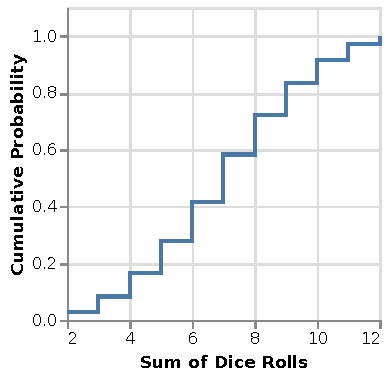
\includegraphics{figures/sum_2_dice_cdf.pdf}
  \caption{$X$ 的 CDF 图象}
  \label{fig:2.1.1}
\end{figure}

注:由于软件限制,各个阶跃点的绘制方式不太规范,实际上从其左侧逼近应该为一个空圈,例如 $F(3)=3/36$ 而不是 $1/36$。另外,$\forall x<2,F(x)=0;\forall x\geq 12,F(x)=1$。
\end{example}

\begin{proposition}
CDF 的性质:
\begin{enumerate}
    \item $F$ 单调递增(未必严格单调递增)
    \item $\lim_{x\rightarrow+\infty}F(x)=1,\lim_{x\rightarrow-\infty}F(x)=0$
    \item $F$ 右连续
\end{enumerate}
\end{proposition}

可以证明,上述三条性质是任意函数 $F:\mathbb{R}\rightarrow\mathbb{R}$ 成为 CDF 的充要条件。

思考:如果我们将 CDF 的定义改为 $P(X<x)$,上述性质会如何变化?

\begin{proposition}
若 $X,Y$ 为随机变量,则 $aX+bY,XY,X/Y\ (\text{需 }Y\neq 0)$ 都是随机变量。一般地,若 $g$ 为可测函数,则 $g(X,Y)$ 是随机变量。
\end{proposition}

\begin{definition}\label{def:2.1.4}
设 $X_1,X_2$ 的 CDF 分别为 $F_1,F_2$,我们称 $X_1$ 与 $X_2$ 同分布,若 $\forall x\in\mathbb{R},F_1(x)=F_2(x)$。
\end{definition}

\begin{proposition}
随机变量 $X_1$ 与 $X_2$ 同分布的一个充要条件是 $\forall \text{ 可测集 }I\subset\mathbb{R},P(X_1\in I)=P(X_2\in I)$。
\end{proposition}

注意,同分布不等价于“同变量”,即两个同分布的变量的取值不一定恒等。

\begin{example}
掷一次硬币,$X$ 表示正面向上次数,$Y$ 表示反面向上次数,显然 $X$ 与 $Y$ 同分布,但取值不等。
\end{example}

\end{document}
